\documentclass{article}

\usepackage{graphicx}
\usepackage{tikz}
\usepackage{tikzsymbols}
\usetikzlibrary{calc,patterns,shapes.geometric}
\pagestyle{empty}
\usepackage[margin=0pt]{geometry}
\geometry{papersize={14in,12in}}

\def\centerarc[#1](#2)(#3:#4:#5){\draw[#1] ($(#2)+({#5*cos(#3)},{#5*sin(#3)})$) arc (#3:#4:#5);}

\begin{document}
	\begin{figure}
		\centering
		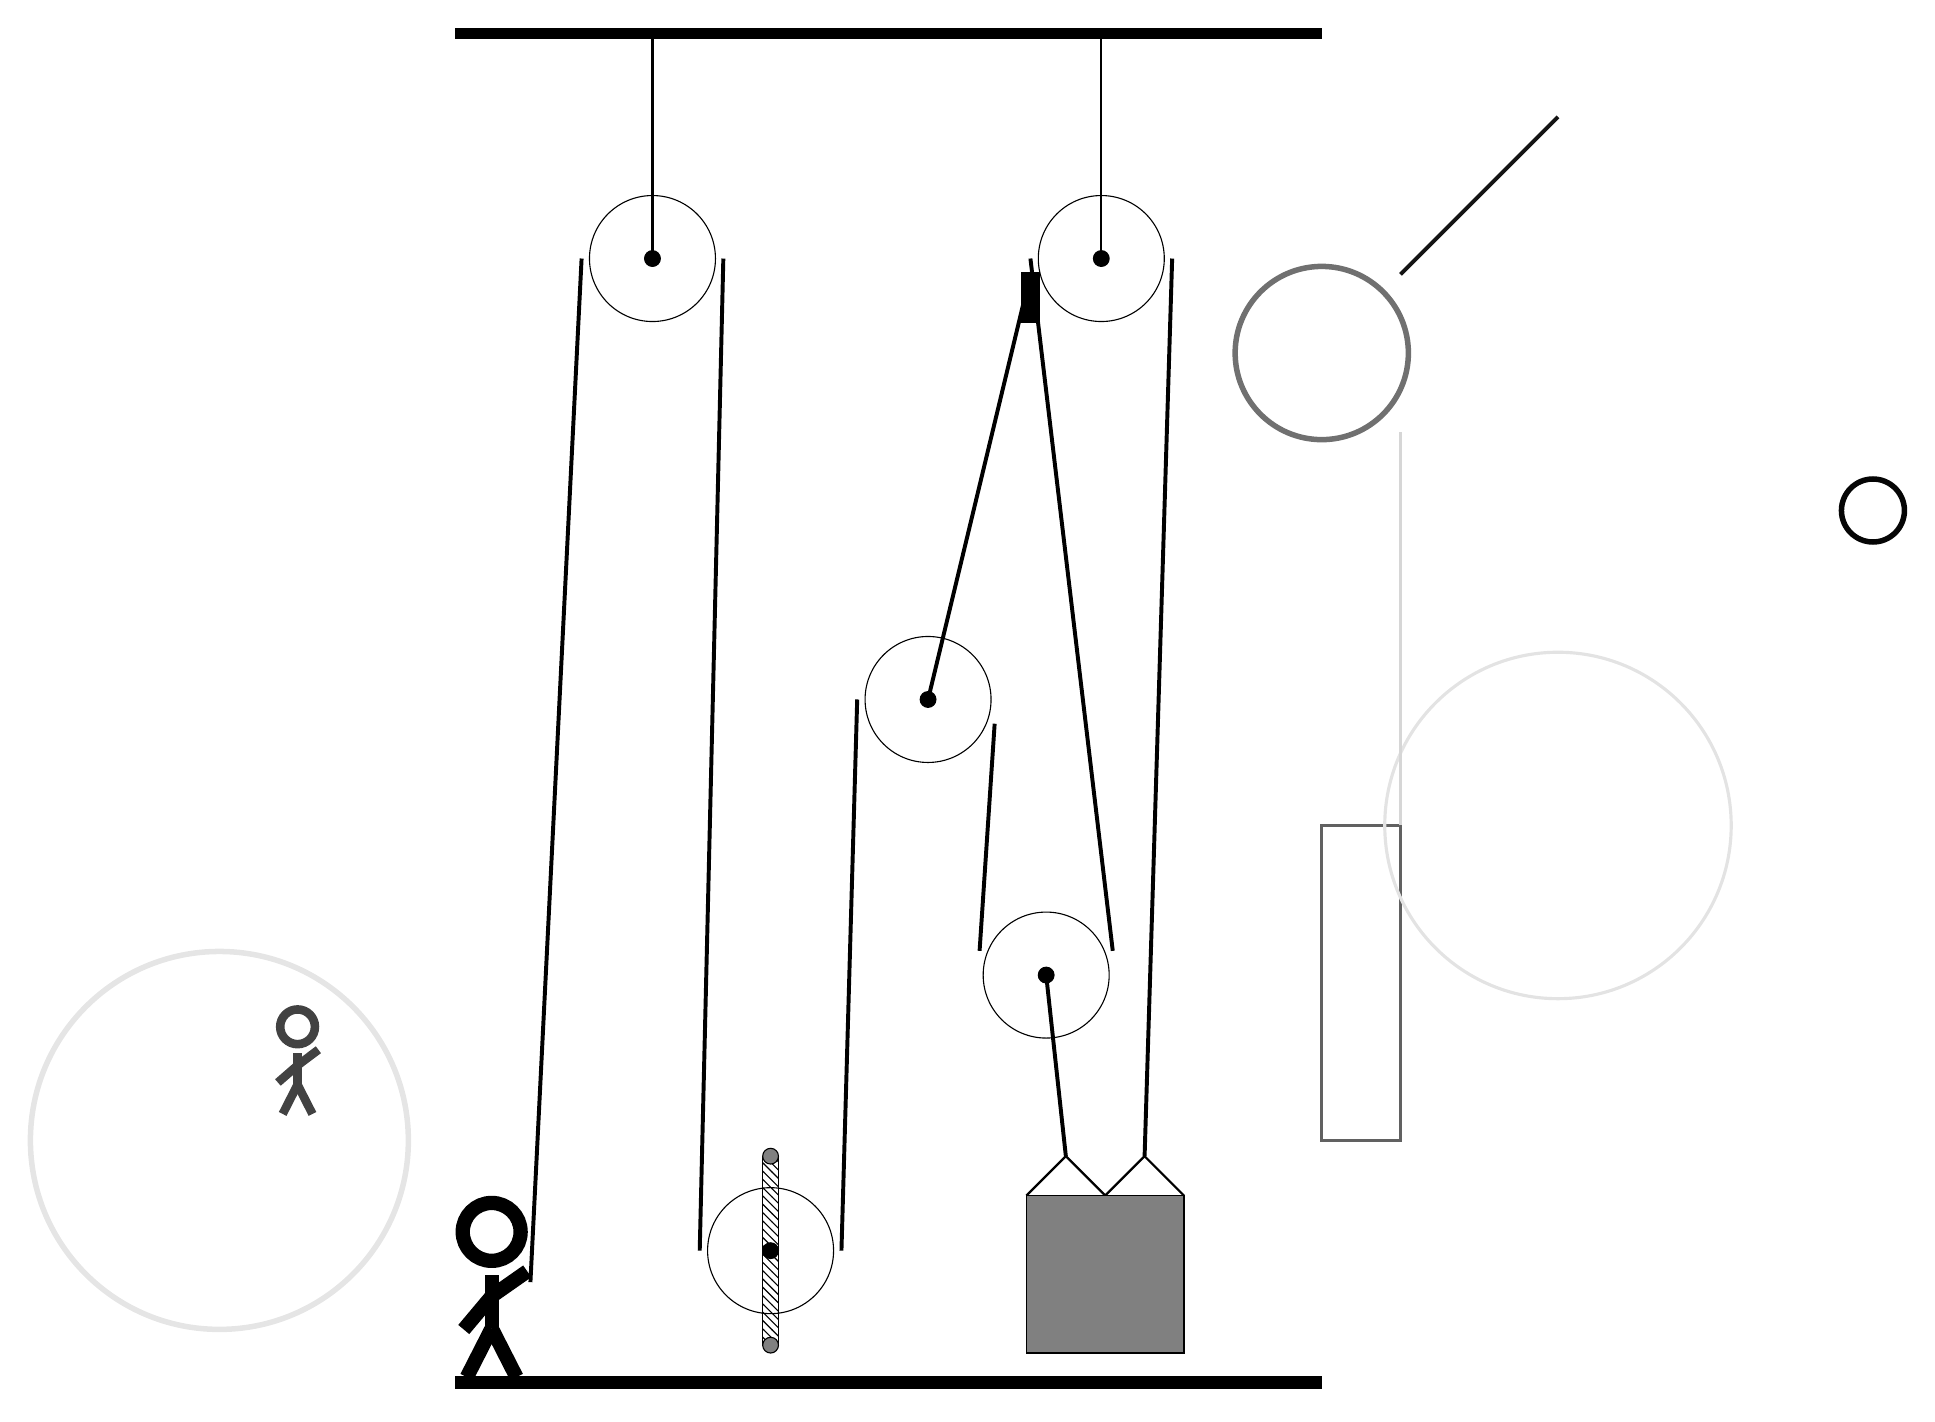
\begin{tikzpicture}
			%%%%% START %%%%%
			
			\draw[fill=black] (-6, 14) rectangle (5, 14.125);
			
			\draw (0, 5.6) circle (0.8);
			\draw[fill=black] (0, 5.6) circle (0.1);
			
			\draw (1.5, 2.1) circle (0.8);
			\draw[fill=black] (1.5, 2.1) circle (0.1);
			
			\draw (2.2, 11.2) circle (0.8);
			\draw[fill=black] (2.2, 11.2) circle (0.1);
			\draw[thick] (2.2, 11.2) -- (2.2, 14);
			
			\draw (-3.5, 11.2) circle (0.8);
			\draw[fill=black] (-3.5, 11.2) circle (0.1);
			\draw[thick] (-3.5, 11.2) -- (-3.5, 14);
			
			\draw (-2, -1.4) circle (0.8);
			\draw[fill=black] (-2, -1.4) circle (0.1);
			\draw[pattern=north west lines, pattern color=black] (-2.1, -0.2) rectangle (-1.9, -2.6);
			\draw[fill=black!50] (-2, -0.2) circle (0.1);
			\draw[fill=black!50] (-2, -2.6) circle (0.1);
			
			\draw [line width=0.7mm, color=black!10](-9, 0) circle (2.4);
			
			\draw[line width=0.4mm, color=black!62] (6, 4) rectangle (5, 0);
			\draw [line width=0.4mm, color=black!11](8, 4) circle (2.2);
			\draw [line width=0.7mm, color=black!98](12, 8) circle (0.4);
			\draw [line width=0.7mm, color=black!56](5, 10) circle (1.1);
			\draw[line width=0.5mm, color=black!16](6, 4) -- (6, 9);
			\node[line width=0.6mm, color=black!74] at (-8, 1) {\Strichmaxerl[6][41][37]};
			\draw[line width=0.5mm, color=black!92](6, 11) -- (8, 13);
			
			\draw[thick]  (1.25, -0.7) -- (1.75, -0.2) -- (2.25, -0.7) -- (2.75, -0.2) -- (3.25, -0.7);
			\draw[fill=black!50] (1.25, -0.7) rectangle (3.25, -2.7);
			\draw[line width=0.5mm] (-5.05, -1.8) -- (-4.4, 11.2);
			\centerarc[line width=0.5mm](-3.5, 11.2)(0:180:0.9);
			\draw[line width=0.5mm] (-2.6, 11.2) -- (-2.9, -1.4);
			\centerarc[line width=0.5mm](-2, -1.4)(180:360:0.9);
			\draw[line width=0.5mm] (-1.1, -1.4) -- (-0.9, 5.6);
			\draw[line width=0.5mm] (0, 5.6) -- (1.3, 11.0);
			\draw[line width=0.5mm, fill=black](1.2, 10.4) rectangle (1.4, 11.0);
			\centerarc[line width=0.5mm](0, 5.6)(-20:180:0.9);
			\draw[line width=0.5mm] (0.8457, 5.2922) -- (0.6543, 2.4078);
			
			\centerarc[line width=0.5mm](1.5, 2.1)(160:380:0.9);
			\draw[line width=0.5mm] (2.3457, 2.4078) -- (1.3, 11.2);
			\draw[line width=0.5mm](1.5, 2.1) -- (1.75, -0.2);
			\centerarc[line width=0.5mm](2.2, 11.2)(0:180:0.9);
			\draw[line width=0.5mm] (3.1, 11.2) -- (2.75, -0.2);
			
			\node at (-5.5, -1.9) {\Strichmaxerl[10][50][35]};
			
			\draw[fill=black] (-6, -3) rectangle (5, -3.15);
			
			%%%%% END %%%%%
		\end{tikzpicture}
	\end{figure}	
\end{document}